\documentclass[11pt]{article}
\usepackage[a4paper,margin=2.5cm]{geometry}
\usepackage[T1]{fontenc}
\usepackage[utf8]{inputenc}
\usepackage{amsmath,amssymb,amsthm}
\usepackage{booktabs,array}
\usepackage{graphicx}
\usepackage{xcolor}
\usepackage[numbers,sort&compress]{natbib}
\usepackage[colorlinks=true,linkcolor=blue!50!black,citecolor=blue!50!black,urlcolor=blue!50!black]{hyperref}

\newtheorem{proposition}{Proposition}
\newtheorem{remark}{Remark}
\newcommand{\qgZ}{qg_Z}
\newcommand{\qgS}{qg_S}
\newcommand{\qgX}{qg_X}
\newcommand{\Tr}{\operatorname{Tr}}

\title{Z-basis metrics for parameterized quantum circuits:\\
exact identities, structural blind spots, pole-damped optimization,\\
and a relaxation-aware entropy benchmark}
\author{Vicente Humberto Monteverde\\
\small Universidad del Museo Social Argentino (UMSA), Argentina\\
\small ORCID 0000-0001-8884-4811}
\date{\small Draft of 23 September 2026; revised 26 September 2026}

\begin{document}
\maketitle

\begin{abstract}
The Qang ($qg$) framework~\cite{monteverde2026qang} expresses single-qubit rotations through two
measurement-level quantities, the polar bias $\qgZ=\langle\sigma_z\rangle$ and the outcome entropy
$\qgS=H(p_0)$. We report results obtained with the open-source reference implementation
\texttt{qang}. First, the two metrics are linked by an exact, branch-free identity,
$\qgS=H\big((1+\qgZ)/2\big)$, which holds for any single-qubit state. Consequently, any new
multi-qubit information must come from the joint outcome distribution. We name the resulting Z-basis total correlation and give its
bounds and its scope: it is not an entanglement measure. Second, we identify exact blind spots:
graph-state entanglement and readout-only dephasing are invisible to every Z-diagonal statistic,
and qg-space updates cannot reach optima outside $[0,\pi]$ because of the $\arccos$ range. On H$_2$
they recover none of the correlation energy. Third, we study a pole-damped gradient step whose
damping schedule is $|d\qgZ/d\theta|$. On a 300-landscape benchmark, H$_2$, and a 4-qubit LiH
Hamiltonian with a mixed $R_y/R_x$ ansatz, it trades 3--20$\times$ more iterations at well-tuned
learning rates for convergence where plain gradient descent diverges. Fourth, as a benchmark, $\qgS$
tracks heavy output probability ($r=-0.93$) and needs no calibration, unlike linear XEB. However,
it is \emph{not} monotonic under amplitude damping: under device-calibrated noise with added idle
relaxation it falls below its own noiseless value. Pairing $\qgS$ with the register-averaged $\qgZ$
removes the ambiguity in 23 of 24 circuits tested. A summary section lists seventeen follow-up
studies (QML encoding, control quantization, noise-type detection, circuit knitting, chemistry,
error mitigation, thermal states, error correction, Hubbard dynamics, constrained QAOA and qubit
characterization), each with its classical or standard control; the symmetry-witness results are
developed in a companion paper. Every number is reproduced by a script and
pinned by a regression test in the public repository.
\end{abstract}

\section{Introduction}

Parameterized quantum circuits are written in angles, but everything a device returns is a
distribution over measurement outcomes. The Qang framework~\cite{monteverde2026qang} makes that
second view the primary one: for a qubit at polar angle $\theta$,
\begin{equation}
  \qgZ(\theta)=\cos\theta=\langle\sigma_z\rangle\in[-1,1],\qquad
  \qgS(\theta)=H\!\left(\cos^2\tfrac{\theta}{2}\right)\in[0,1],
\end{equation}
with $H(p)=-p\log_2p-(1-p)\log_2(1-p)$. This paper collects results obtained with the reference
implementation \texttt{qang}, with the aim of stating where the metrics are exact, where they are
blind, and where they mislead. Section~\ref{sec:identities} gives exact identities,
Section~\ref{sec:blind} the structural blind spots, Section~\ref{sec:opt} a pole-damped optimizer
on molecular Hamiltonians, and Section~\ref{sec:bench} the behavior of $\qgS$ as a benchmark,
including a device-calibrated validation. Section~\ref{sec:further} summarizes later results, and
Section~\ref{sec:limits} lists the limitations together.

All results are produced by scripts in the \texttt{examples/} folder of the repository and pinned
by regression tests (Section~\ref{sec:code}). Molecular Hamiltonians were derived once with
PySCF~\cite{sun2018pyscf} and are hard-coded, so neither PySCF nor qiskit-nature is a dependency.

\section{Exact identities}\label{sec:identities}

\subsection{A branch-free link between \texorpdfstring{$\qgZ$}{qgZ} and \texorpdfstring{$\qgS$}{qgS}}

Inverting $\qgS\mapsto\theta$ requires choosing a half-domain, because $\qgS(\theta)=\qgS(\pi-\theta)$.
The opposite direction needs no choice.

\begin{proposition}\label{prop:identity}
For any single-qubit density matrix $\rho$, with $\qgZ=\Tr(\rho\sigma_z)$ and $\qgS=H(\langle0|\rho|0\rangle)$,
\begin{equation}
  \qgS=H\!\left(\frac{1+\qgZ}{2}\right),\qquad
  \frac{d\,\qgS}{d\,\qgZ}=\frac12\log_2\frac{1-\qgZ}{1+\qgZ}.
\end{equation}
\end{proposition}
\begin{proof}
$\qgZ=p_0-p_1=2p_0-1$ with $p_0=\langle0|\rho|0\rangle$; substitute into $H(p_0)$ and differentiate.
\end{proof}

The proof uses only the Z-diagonal population. The identity therefore holds however the state was
prepared ($R_y$, $R_x$, a noisy channel, or a partial trace of a larger register), and the tests check it on random
Haar states. The derivative diverges at $\qgZ=\pm1$. This is the entropy-side counterpart of the
Jacobian singularity $d\theta/d\qgZ=-1/\sin\theta$.

\subsection{Z-basis total correlation}

Applied to each reduced single-qubit state, Proposition~\ref{prop:identity} makes the per-qubit
$\qgZ$ profile and the per-qubit marginal $\qgS$ two encodings of the same information. Anything
new about an $n$-qubit register must come from the joint distribution of the Z-basis outcomes
$X_1,\dots,X_n$. We define
\begin{equation}
  C_Z(\rho)=\sum_{i=1}^n H(X_i)-H(X_1,\dots,X_n),
\end{equation}
Watanabe's total correlation~\cite{watanabe1960} of the outcomes. For $n=2$ it equals the mutual
information. By subadditivity, $0\le C_Z\le n-1$ bits, with $C_Z=0$ iff the outcomes are
independent. Product states give 0, Bell states 1 and GHZ$_n$ states $n-1$ (the maximum).

\begin{remark}[Scope]
$C_Z$ is a classical correlation measure and is not a witness of entanglement in either direction.
The separable mixture $\tfrac12(|00\rangle\langle00|+|11\rangle\langle11|)$ has $C_Z=1$, as does a
Bell state. Every graph state has $C_Z=0$ (Section~\ref{sec:blind}).
\end{remark}

\section{Structural blind spots}\label{sec:blind}

\paragraph{Graph states.} A graph state~\cite{hein2004graph} is $H^{\otimes n}$ followed by CZ gates.
$H^{\otimes n}$ makes every $|\text{amplitude}|^2$ equal to $2^{-n}$, and CZ is diagonal. For every
graph, therefore, each qubit has $\qgZ=0$, the joint $\qgS$ is maximal, and $C_Z=0$. The entanglement,
certified independently through the stabilizers $X_i\prod_{j\in N(i)}Z_j$, lives entirely in phases.

\paragraph{Readout dephasing.} Dephasing preserves the diagonal of $\rho$. Applied only before
measurement, it therefore leaves $\qgS$ exactly unchanged at every strength, including full
dephasing (checked to machine precision on a 4-qubit Quantum Volume circuit). The same channel
applied \emph{inside} the circuit is visible: later entangling gates turn the lost coherence into
randomized populations, and $\qgS$ rises monotonically.

\paragraph{The $\arccos$ range.} A qg-space parameter update is mapped back through
$\theta=\arccos(\qgZ)\in[0,\pi]$. On the H$_2$ Hamiltonian (0.735~\AA, STO-3G, two qubits after
parity reduction), the single-excitation optimum lies at $\theta\approx-0.22$. Starting from
Hartree--Fock, raw, clipped and Tikhonov-regularized qg-space descent all stop at exactly the
Hartree--Fock energy ($-1.1169990$~Ha, error $2.0\times10^{-2}$~Ha). They recover none of the
correlation energy, whereas $\theta$-space descent reaches the FCI energy to $10^{-9}$~Ha.
Regularizing the Jacobian cannot fix this, because the limit comes from the range of $\arccos$,
not from its derivative.

\section{Pole-damped gradient descent}\label{sec:opt}

To keep updates in $\theta$-space while still using the pole geometry, we damp each parameter's
step by $|d\qgZ/d\theta_i|$, floored at $\varepsilon$:
\begin{equation}
  \theta_i\leftarrow\theta_i-\eta\,\max(|\sin\theta_i|,\varepsilon)\,\frac{\partial E}{\partial\theta_i}.
\end{equation}
This is position-dependent trust-region damping in the Levenberg--Marquardt
tradition~\cite{levenberg1944,marquardt1963}. It is not a new class of optimizer; the only
framework-specific element is that the schedule is derived from the geometry rather than tuned.
Because the factor depends only on populations, and $R_x(\theta)|0\rangle$ and $R_y(\theta)|0\rangle$
have identical populations, it applies unchanged to either axis. We use $\varepsilon=0.05$ throughout;
results are insensitive to this choice.

\paragraph{Random landscapes.} For 300 random landscapes $E=h_z\cos\theta+h_x\sin\theta$ per
learning rate, started near a pole (Table~\ref{tab:robust}), damping costs a few percent of success at a safe
rate. At $\eta=1$ it succeeds in 100\% of cases versus 77\%, and at larger rates it succeeds 2.5--5 times more often.
The cost is a trapping mode, in which the optimizer oscillates at its starting pole; it reaches
6.7\% at $\eta=10$.

\begin{table}[t]
\centering\small
\caption{Success rates over 300 random one-qubit landscapes per learning rate, started near a pole.}
\label{tab:robust}
\begin{tabular}{lcccccc}
\toprule
$\eta$ & 0.3 & 1.0 & 2.0 & 3.0 & 5.0 & 10.0\\
\midrule
plain success & 0.997 & 0.773 & 0.187 & 0.087 & 0.057 & 0.027\\
damped success & 0.963 & 1.000 & 0.477 & 0.357 & 0.253 & 0.130\\
damped trapped & 0.017 & 0.000 & 0.030 & 0.023 & 0.040 & 0.067\\
\bottomrule
\end{tabular}
\end{table}

\paragraph{H$_2$, two coupled parameters.} Ansatz $R_y(\theta_0)\otimes R_y(\theta_1)$ followed by CX; the optimum
has $\theta_0=\pi$ (a pole). From $(1.0,10^{-6})$, damping needs about $3\times$ more steps to reach
chemical accuracy at safe rates (603 vs.\ 196 at $\eta=0.05$). At $\eta=2.5$, 3 and 4, plain
descent never reaches chemical accuracy, while the damped version reaches the FCI energy in 10, 8 and
6 steps.

\paragraph{LiH, mixed axes.} LiH at 1.5459~\AA\ (STO-3G, 2 electrons in 3 spatial orbitals, parity
mapping) gives 4 qubits and 52 Pauli terms, the scale of early hardware VQE
work~\cite{omalley2016,kandala2017}. The ansatz is $R_y(\theta_0)$, $R_y(\theta_1)$ on the occupied
orbitals and $R_y(\theta_2)$, $R_x(\theta_3)$ on the virtual ones, followed by CX$(2\!\to\!0)$ and CX$(3\!\to\!1)$. At
$(\pi,\pi,0,0)$ its state has overlap 1 with qiskit-nature's Hartree--Fock circuit. All four
optimal parameters lie within 0.04~rad of a pole, which makes the cost larger than for H$_2$: 355
vs.\ 17 steps at $\eta=0.3$. The benefit is also larger (Table~\ref{tab:lih}). The $R_x$ phase is
physical: after the CX it changes the energy relative to $R_y$ at the same angle, although the
single-qubit populations are identical.

\begin{table}[t]
\centering\small
\caption{LiH, start $(\pi,\pi,10^{-6},10^{-6})$: steps to sustained convergence ($10^{-5}$~Ha) to the
ansatz optimum $-0.0440152$~Ha (active-space electronic energy; HF $-0.0437813$, FCI $-0.0448309$).}
\label{tab:lih}
\begin{tabular}{lccccccc}
\toprule
$\eta$ & 0.3 & 1.0 & 2.0 & 2.5 & 4.0 & 7.0 & 10.0\\
\midrule
plain $\theta$ & 17 & 5 & never & never & never & never & never\\
pole-damped & 355 & 106 & 53 & 42 & 26 & 15 & 10\\
\bottomrule
\end{tabular}
\end{table}

\section{\texorpdfstring{$\qgS$}{qgS} as a benchmark}\label{sec:bench}

\paragraph{Heavy output probability and XEB.} On 10 random 4-qubit Quantum Volume
circuits~\cite{cross2019} mixed with global depolarizing noise, $\qgS$ and heavy output probability
have Pearson $r=-0.926$ over 110 points. Linear XEB~\cite{arute2019} has a noiseless value $A-1$,
with $A=2^n\sum_xp(x)^2$ ranging from 1.23 to 2.33 on the same circuits family ($n=3$--6), so it needs
circuit-specific calibration; $\qgS$ does not. Conversely, XEB's estimator is a sample mean and
is unbiased at any shot count, while the plug-in entropy is biased low (bias $-0.054$ at 50 shots
on 4 qubits). The Miller--Madow correction~\cite{miller1955} reduces that bias about fivefold.

\paragraph{Amplitude damping breaks monotonicity.} The reading ``more noise $\Rightarrow$ higher
$\qgS$'' holds only for channels whose fixed point is maximally mixed. With amplitude damping
applied after every two-qubit block (Fig.~\ref{fig:t1}a), $\qgS$ rises from 0.919 to 0.983 at
$\gamma=0.1$ and then falls to 0 at $\gamma=1$. At $\gamma=0.4$ it reads 0.918, almost the noiseless
value.

\paragraph{The fix: register-averaged $\qgZ$.} The mean $\bar{\qgZ}=\frac1n\sum_i\Tr(\rho_i\sigma_z)$
is pulled towards 0 by unital noise and towards $+1$ by relaxation. At $\gamma=0$ and $0.4$ the pairs
$(\qgS,\bar{\qgZ})$ are $(0.919,-0.029)$ and $(0.918,+0.310)$. $\bar{\qgZ}$ rose monotonically along a 21-point
$\gamma$ grid in 23 of 24 circuits ($n=3,4,5$; seeds 0--7); the exception dips by 0.015 before
rising. $\bar{\qgZ}$ is linear in $\rho$, so its estimator from counts is an exact sample mean
(Appendix~\ref{app:riesz}).

\paragraph{Device-calibrated validation.} We ran the same circuit through Qiskit Runtime on the
\texttt{fake\_brisbane} backend, a simulator whose noise model is built from a real IBM device's
calibration data. An idle delay before readout served as a T1 knob (Fig.~\ref{fig:t1}b). Heavy output probability
fell monotonically (0.685 to 0.448) and $\bar{\qgZ}$ rose monotonically ($-0.036$ to $+0.370$). $\qgS$
rose to 0.977 at 50~$\mu$s and then fell to 0.892 at 200~$\mu$s, below its noiseless value of 0.919.
Read on its own, $\qgS$ would rank the most relaxed operating point as the least noisy.

The same script evaluated the LiH ansatz without error mitigation. The raw error was $+0.036$~Ha
at Hartree--Fock and $+0.035$~Ha at the optimum. This is about $20\times$ chemical accuracy and
about $150\times$ the 0.23~mHa difference the optimizer resolves noiselessly. A hardware run of
this VQE therefore needs mitigation first.

\begin{figure}[t]
\centering
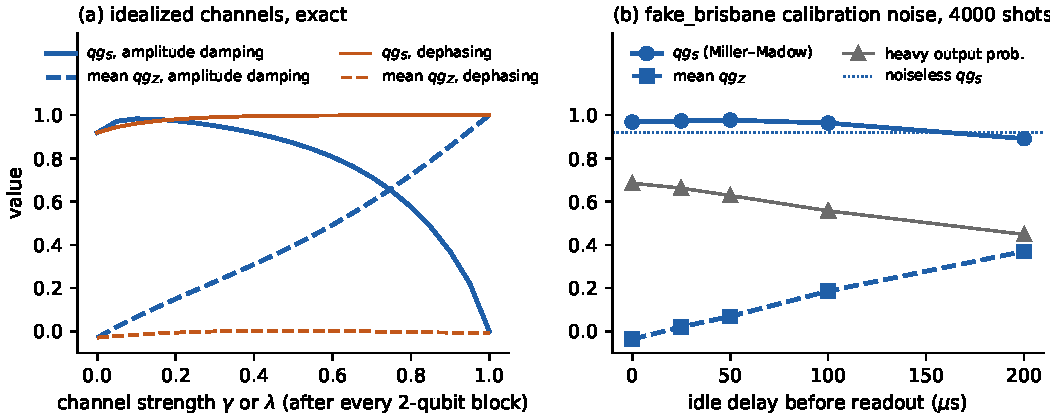
\includegraphics[width=\linewidth]{fig_t1.pdf}
\caption{(a) 4-qubit Quantum Volume circuit, exact density-matrix simulation with amplitude damping
or dephasing after every two-qubit block. $\qgS$ is non-monotonic under amplitude damping, while the mean
$\qgZ$ separates the regimes. (b) The same circuit under \texttt{fake\_brisbane}
calibration noise with an idle delay before readout. Heavy output probability and mean $\qgZ$ are
monotonic; $\qgS$ falls below its noiseless value (dotted).}
\label{fig:t1}
\end{figure}

\paragraph{Randomized benchmarking and ZNE.} Under per-gate depolarizing noise $p$, the RB survival
signal is exactly $\qgZ(m)=(1-p)^{m+1}$, identical across random Clifford sequences to 10 digits
in our runs~\cite{magesan2011}. For zero-noise extrapolation~\cite{temme2017}, extrapolation in
$\qgZ$-space is exact for Bloch-vector shrinkage but biased ($1.8\times10^{-3}$) for coherent angle drift;
$\theta$-space shows the reverse. One should extrapolate in whichever space makes the noise linear.
In barren-plateau settings~\cite{mcclean2018,cerezo2021}, regularized qg-space gradients keep the
exponential variance decay, and raw qg-space gradients still diverge at the poles.

\section{Further results (summary)}\label{sec:further}

After the first draft, the same code base was used for seventeen further studies. Each compares a
qg-based choice with the standard one and with a classical control, and each is documented in
\texttt{RESEARCH\_NOTES.md} (section numbers below) with a script and pinned tests.
Table~\ref{tab:further} lists them. The column ``gain'' states against what the qg choice wins,
if at all. None of them is a quantum advantage over classical computation. Where a classical
method was run, it matched or beat the quantum model at these sizes. The symmetry-witness studies
(§20, §21, §24, §28--§31) are developed in a companion paper~\cite{monteverde2026witness}.

\begin{table}[t]
\centering\footnotesize
\caption{Follow-up studies (section numbers of \texttt{RESEARCH\_NOTES.md}).}
\label{tab:further}
\begin{tabular}{>{\raggedright\arraybackslash}p{0.9cm}>{\raggedright\arraybackslash}p{4.0cm}>{\raggedright\arraybackslash}p{5.8cm}>{\raggedright\arraybackslash}p{3.2cm}}
\toprule
§ & topic & main number & gain \\
\midrule
15 & natural gradient, cut cost, few-shot $\qgZ$ & QFI $=1/(1-\qgZ^2)$; cut $\gamma=1+2\sqrt{1-\qgZ^2}$; Haar prior 92\% vs 8\% coverage near a pole & closed forms; vs delta method \\
16, 19 & QML encoding $\theta=\arccos x$ & Chebyshev models fit polynomials to $10^{-13}$ vs $5\times10^{-5}$; $\sim10\times$ with shots & vs angle encoding~\cite{schuld2021}; classical Chebyshev fit wins \\
17 & control grid uniform in $\qgZ$ & probability error $\pi/2$ smaller; distribution loading TVD lower in 43/45 cases & vs $\theta$ grid; loses on fidelity near poles \\
18 & T1 vs unital noise from counts & accuracy 0.88--0.91 vs 0.70--0.76 (XEB, HOP), strong noise only & vs XEB/HOP \\
20 & IonQ noise models & H$_2$ + $\qgZ$ filter $\sim$12 vs $\sim$30~mHa, 2--3\% shots dropped & vs readout mitigation \\
21 & H$_2$ electron-number witness & 5.5 vs 18~mHa (HF 20.3); $11\times$ below HF at 2.5~\AA; no gain on 6-qubit LiH & vs readout mitigation, HF \\
22 & ODE solver~\cite{kyriienko2021} & exponential decay up to $17\times$ better; not in general & vs angle encoding; spectral method wins \\
23 & local cost $(1-\bar{\qgZ})/2$ & gradient variance $5600\times$ larger at 12 qubits; light cone trains 100 qubits classically & vs global cost~\cite{cerezo2021}; classically simulable~\cite{cerezo2023simulability} \\
24 & $\qgZ$ filter vs ZNE by noise type & witness predicts when the filter works; ZNE + filter 2.0~mHa on \texttt{fake\_brisbane} & complementary to ZNE \\
25 & thermal qubit, $\qgZ=\tanh\beta h$ & optimal thermometer $\qgZ\operatorname{artanh}\qgZ=1$~\cite{correa2015} & none (prior, not qg) \\
26 & which gates to cut & exact optimum over 3795 partitions; $2\times$ fewer shots than counting & vs angle-blind rules; same as \texttt{find\_cuts} \\
27 & repetition code choice under T1 & $\qgZ$+$\qgX$ policy regret 2.7\% vs 46--258\% & decision rule \\
28 & spin-resolved filters & 23.2 $\to$ 14.7~mHa under depolarizing noise; none on \texttt{fake\_brisbane} & conditional \\
29 & 1D Hubbard, 8 qubits & ZNE + spin filters 6--9$\times$ below raw; wall at $\geq$188 ECR & vs raw, ZNE \\
30 & QAOA, exactly $K$ & filter doubles $P(\mathrm{opt})$ of XY-QAOA; penalty QAOA $\approx$ random guess & vs QAOA; greedy wins \\
31 & qubit characterization & unbiased $T_\mathrm{eff}$ ($\pm1$~mK) and readout error, where the standard suite reads 0~K & vs standard calibration \\
\bottomrule
\end{tabular}
\end{table}

\section{Limitations}\label{sec:limits}

(i) The Jacobian singularity at $\theta\in\{0,\pi\}$; regularization costs exactness there.
(ii) The $\arccos$ range: qg-space updates cannot reach $\theta<0$.
(iii) Z-basis blindness to phase-encoded entanglement and to readout dephasing.
(iv) $C_Z$ is not an entanglement measure.
(v) $\qgS$ is not monotonic under T1. The pair $(\qgS,\bar{\qgZ})$ fixes this empirically, in
23 of 24 circuits, not provably.
(vi) Finite-shot bias of $\qgS$.
(vii) Pole damping costs iterations and has a trapping mode.
(viii) All device results, here and in the follow-up studies, are calibration-based or
vendor-model simulations. Runs on real hardware (\texttt{--mode ibm}, IonQ) are prepared but have
not yet been performed.

\section{Code availability}\label{sec:code}

The library, every example, and the regression tests pinning every number above (809 tests at
the time of this revision) are available at
\url{https://github.com/Viny2030/qang} (MIT license). Figure~\ref{fig:t1} is regenerated by
\texttt{manuscript/make\_figures.py}. Derivations with additional detail are in
\texttt{RESEARCH\_NOTES.md}.

\section*{Acknowledgments and use of AI tools}
Generative AI tools (Anthropic Claude 3.5 Sonnet and Claude Opus 5.5; OpenAI GPT-4o) assisted with
code generation and refactoring, test expansion, numerical experiments, and drafting of this text.
The author framed the research questions, made the design decisions, and reviewed, edited and
validated all AI-assisted output, including every derivation and number reported here.

\appendix
\section{Riesz--Fr\'echet and why \texorpdfstring{$\qgZ$}{qgZ} is the canonical linear readout}\label{app:riesz}

Operators on $\mathbb{C}^{2^n}$ form a Hilbert space under $\langle A,B\rangle=\Tr(A^\dagger B)$.
By the Riesz--Fr\'echet representation theorem~\cite{riesz1907,frechet1907}, every linear functional
on it has the form $\rho\mapsto\Tr(O\rho)$ for a unique $O$. In finite dimension this is elementary
linear algebra, so the appendix records a foundation rather than a new result. The functional
$\rho\mapsto\qgZ(\rho)$ is represented by $\sigma_z$, and $\bar{\qgZ}$ by $\frac1n\sum_iZ_i$.
Every linear readout, including linear XEB, has this form and hence an unbiased sample-mean
estimator. $\qgS$ is strictly concave in $\rho$, so no operator represents it, and its plug-in
estimator is biased by Jensen's inequality. By Proposition~\ref{prop:identity}, $\qgS$ is a fixed
scalar function of the linear quantity $\qgZ$, so it carries no information about a single qubit
beyond what $\sigma_z$ extracts. (Riesz's 1918 lemma on almost-orthogonal vectors concerns
infinite-dimensional spaces and plays no role here.)

\bibliographystyle{unsrtnat}
\bibliography{refs}
\end{document}
